\documentclass[border=3pt,tikz]{standalone}
\usepackage[utf8]{vietnam}
\usetikzlibrary{calc,angles,intersections,shapes.geometric,arrows,decorations.markings,arrows.meta,patterns.meta,patterns}
\usepackage{tikz-3dplot,pgfplots}
\pgfplotsset{compat=1.15}
\usepgfplotslibrary{polar}
\usepackage{amsmath}
\begin{document}
	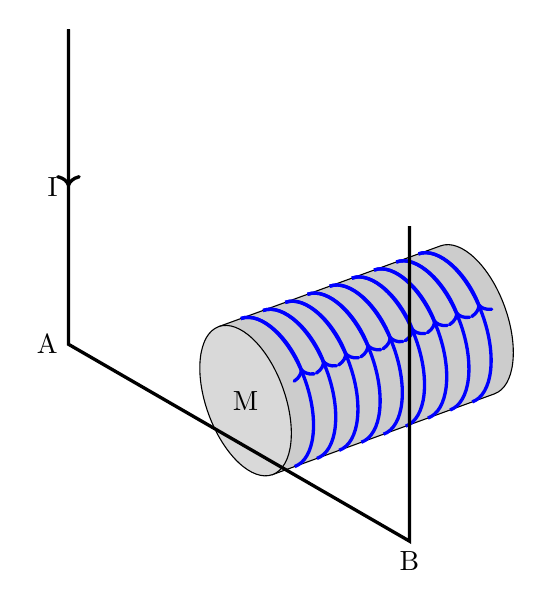
\begin{tikzpicture}[rotate=20]
	\draw[fill=gray!40](0,1)--++(0:3)arc(90:-90:0.5cm and 1cm)--++(180:3)--cycle;
	\draw[fill=gray!30] (0,0) ellipse (0.5cm and 1cm);
	\foreach \x in {0.3,0.6,...,2.8}
	{\draw [very thick,blue] (\x,1) arc(90:-90:0.5cm and 1cm);
		\draw [very thick,blue,-<] (\x,1) arc(90:0:0.5cm and 1cm);}
	\draw[very thick](-0.5,5.2)--++(-110:4)node[left]{A}--++(-50:5)node[below]{B}--++(70:4);
	\draw[very thick,->](-0.5,5.2)--++(-110:2)node[left]{I};
	\node at (0,0){M};
\end{tikzpicture}
\end{document}